% Introduction

\subsection{Related Work}


\subsection{Completed Work}
From countries, states, and regions to neighborhoods, local meeting houses, or churches, the places we live and visit are tightly connected to our identities.
Location information gathered about an individual over time can reveal much more than a home location.
In fact, patterns in human mobility can reveal more private components of an individual's 
blah, such as their race, gender, or economic status.

In this section, I will discuss two works which explore these issues.
Both rely on a dataset connecting images to mobility through geotagged photos on the image-sharing site Instagram.
In the first, we label faces for gender, race, and other attributes, and explore whether these features can be inferred from locations visited.
In the second, we evaluate the use computational vision techniques to scale up the use of Instagram to connect mobility to demographics for an ``automated census".


\subsubsection{I Don’t Have a Photograph But You Can Have My Footprints}




\subsubsection{Scaling up the Census with Social Media}

% \begin{abstract}
The growth of publicly available online information from social networks provides many opportunities to demographic researchers.
However, this data is often messy and unlabeled, causing researchers to need to label profiles with demographics.
This labelling is either done manually, a costly and time-consuming process, or done via automated algorithms.
The inputs to these algorithms have previously been text-based, taking a user's posts or name as input.
Techniques involving computational vision have been left unused, due to a lack of training data from users and problems of low accuracy.

In this work, we evaluate the feasibility of combining modern facial recognition techniques with publicly available social media images to conduct large scale demographic research.
We find that facial recognition can be used to label the gender and race of social media profiles with high precision and recall.
We further investigate factors that improve or hinder demographic labeling accuracy, showing a disparity between the accuracy of labelings of profiles of racial majority and minorities.
We conclude with ideas for future improvements and research.
% \end{abstract}


\textbf{Introduction} \\
The great wealth of publicly available, online social networking data has been a boon to demographic research due to its richness and scale.
Never before has such an amount of human behavioral data been easily obtained and analyzed.
However, before this data can be used to study demographics, each user must be labeled with demographic categorizations. 
This poses a particular challenge in many online social networking (OSN) sites which often do not display or even obtain the demographic information of its users.

To meet this need, researchers in the past have tried a variety of techniques.
Manual labeling by individually investigating each profile is costly in terms of time, effort, and money.
Some studies have relied on data provided by marketing companies or data aggregators~\cite{Goel:2012ut, biinferring}.
Due to cost and issues of reproducibility, these sources of data are not available to all researchers.

To improve the scale of labeling while keeping costs low, researchers have used automated techniques which range in complexity.
For example, researchers have compared public names to lists of gender and ethnicity for those names~\cite{mislove-2011-twitter, ICWSM101534}.
Others have run simple algorithms on location data~\cite{riederer2015cosn} or more sophisticated techniques that incorporate text posted and the structure of a user's social network~\cite{ICWSM112886, pennacchiotti2011democrats}.
These techniques offer some promise but often are not very robust and may not be applicable to OSNs with little textual interaction, such as Instagram.

% TODO: This doesn't really fit.
Researchers that use these automated tools for labeling must be wary of introducing algorithmic bias.
As argued in~\cite{Selbst:2014wi}, data mining can lead to biased results.
Algorithms that have disparate accuracies in demographic labeling could cause erroneous or biased results.

In the past, computational vision has not been an effective technique for labeling the demographics of social media users, due to three issues: (1) CV algorithms being too slow, (2) CV algorithms having low accuracy, (3) a lack of publicly available and uniformly popular photographs as data.
However, in recent years, face recognition tools have improved to become both highly accurate and efficient.
Additionally, the social network Instagram has made image-sharing a ubiquitous activity across most of the developed and much of the developing world.

Instagram is an interesting social network to study for a variety of reasons.
With over 400 million users at the time of writing, over 5\% of the world's population user Instagram.
A quarter of these users are based inside the United States, meaning that nearly 1 in 3 United States citizens uses Instagram~\cite{igstats}.
Beyond its scale, Instagram is interesting for its content.
Photographs are extremely rich, capturing information on all sorts of human activities and interactions.
Although images can be more difficult to analyze than text, the research community has begun to study Instagram behavior~\cite{hu2014we, bakhshi2014faces} and even selifes~\cite{souza2015dawn}.

In this paper, we show that a popular face recognition API can be used to scalably and accurately learn the gender and race of Instagram users.
We use a dataset of 200 Instagram profiles, labeled for gender and race, to analyze the practicality and accuracy of facial recognition, achieveing 86\% accuracy for gender and 82\% accuracy for race in a limited setting.
We additionally explore the accuracy of labeling different demographics as the amount of data increases, showing some concerns about algorithmic bias.
We conclude with ideas for future work.

\textbf{Data} \\
\textbf{Collection} \\
We used a subset of the Instagram data collected in~\cite{riederer2015cosn}.
In this paper, the authors gathered the metadata (such as time of photo, URL of image, tags, location, etc.) for all photographs of a ``root" user, Kevin Systrom, the founder of Instagram.
They then collected the user IDs of users who had commented or liked his photos, gathered their metadata, and repeated this process.
A subset of these users were then selected based on geography-- only users with more than half of their photographs taken in Los Angeles or New York were kept.

Two research assistants labeled a randomly selected subset of 200 of these profiles for gender and race.
After filtering for private, deleted, or business profiles, 172 profiles remained.
For gender, the labelers selected from male, female, or other.
In practice, only the male or female categories ended up being used.
For race, a subset of the United States Census categories were used: White, Black, Hispanic, Asian, and other.
The labelers agreed on gender for 170 of the profiles and for race on 147.
The process resulted in 76 profiles as Male and 94 as Female.
For race, 75 were labeled White, 28 as Hispanic, 27 as Black, 16 as Asian, and 1 as other.

Our next step was to recognize and label faces present in these Instagram users' profiles using computer vision.
For this task, we used Face++~\cite{faceplusplus}, a popular API with reported high degress of accuracy~\cite{bakhshi2014faces}.
In addition to recognizing faces within images, Face++ labels race from {White, Black, Asian} with a \emph{confidence score} 0-100, gender from {Male, Female} with a \emph{confidence score} 0-100.

For each user in this data set, we gathered the metadata of the first 100 Instagram photos.
Each image was then analyzed with the Face++ API.
Face++ only requires that a URL to an image is passed to it.
Therefore, this methodology does \emph{not} require that any images are downloaded, uploaded, or even viewed by a human labeler.
Note that not every photo on Instagram has a face in it, and some have more than one.

This resulted in 170 distinct users with at least one or more face present in their photos.
We obtained 5,272 photos and depicting 12,143 faces. 
Additionally, for each user, we passed the URLs for their profile pictures.
A total of 70 users had profile pictures in which Face++ could detect a face.
73 faces were found: 2 profiles pictures had 2 faces in them.

\textbf{Description}


\begin{figure}[t]
  \centering
  \begin{subfigure}[b]{.21\textwidth}
    \centering
    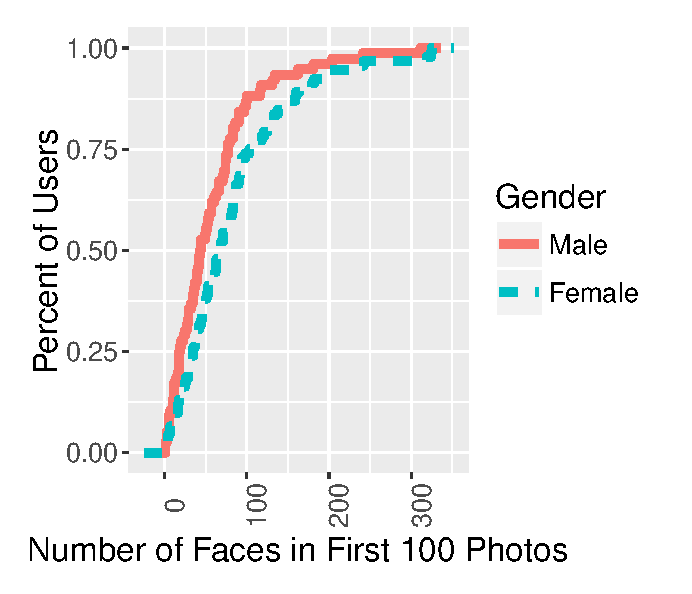
\includegraphics[width=\linewidth]{fig/census/face_cdf_gender.eps}
    \caption{}
    \label{fig:face_cdf_gender}
  \end{subfigure}
  \begin{subfigure}[b]{.21\textwidth}
    \centering
    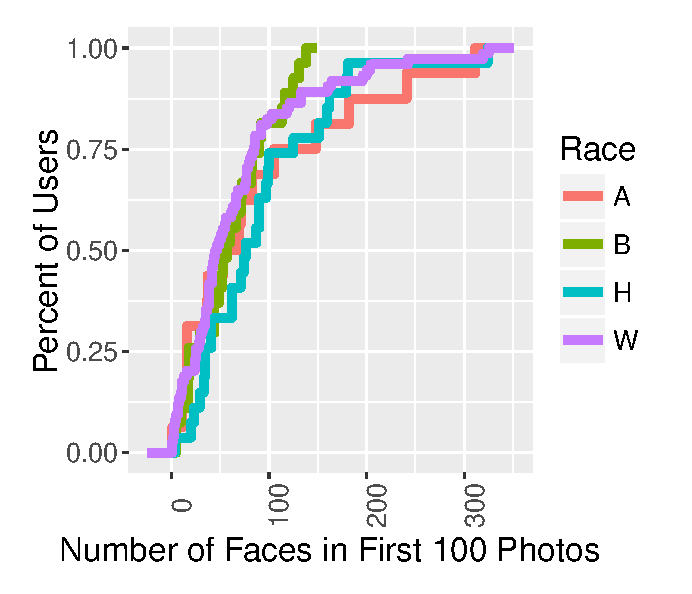
\includegraphics[width=\linewidth]{fig/census/face_cdf_race.eps}
    \caption{}
    \label{fig:face_cdf_race}
  \end{subfigure}
  \caption{}
  \label{fig:face_cdf}
\end{figure}

\begin{figure}[t]
  \centering
  \begin{subfigure}[b]{.21\textwidth}
    \centering
    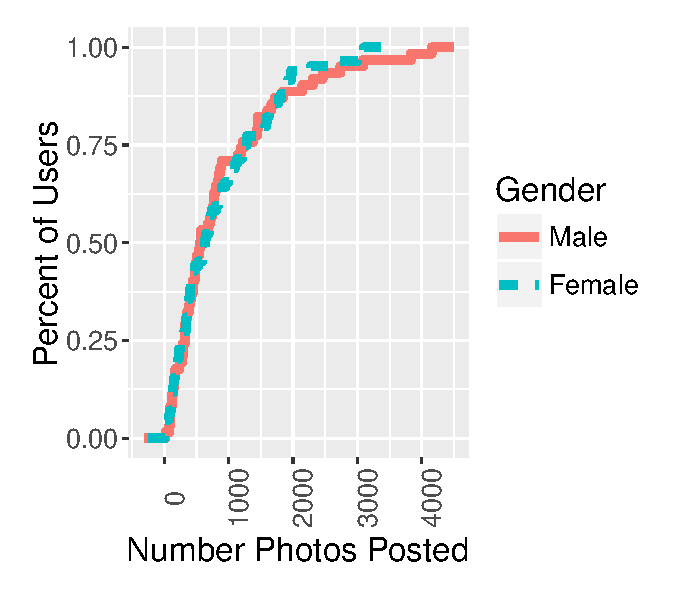
\includegraphics[width=\linewidth]{fig/census/numphoto_cdf_gender.eps}
    \caption{}
    \label{fig:numphoto_cdf_gender}
  \end{subfigure}
  \begin{subfigure}[b]{.21\textwidth}
    \centering
    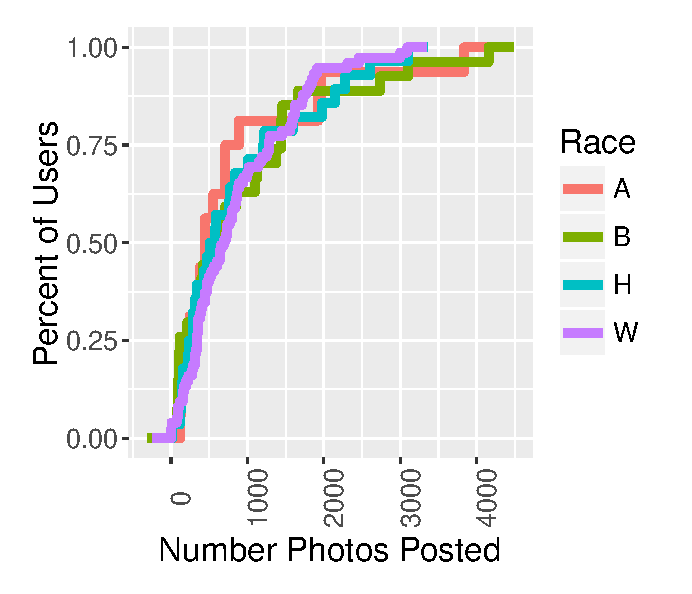
\includegraphics[width=\linewidth]{fig/census/numphoto_cdf_race.eps}
    \caption{}
    \label{fig:numphoto_cdf_race}
  \end{subfigure}
  \caption{}
  \label{fig:numphoto_cdf}
\end{figure}


\begin{figure}[t]
  \centering
  \begin{subfigure}[b]{.21\textwidth}
    \centering
    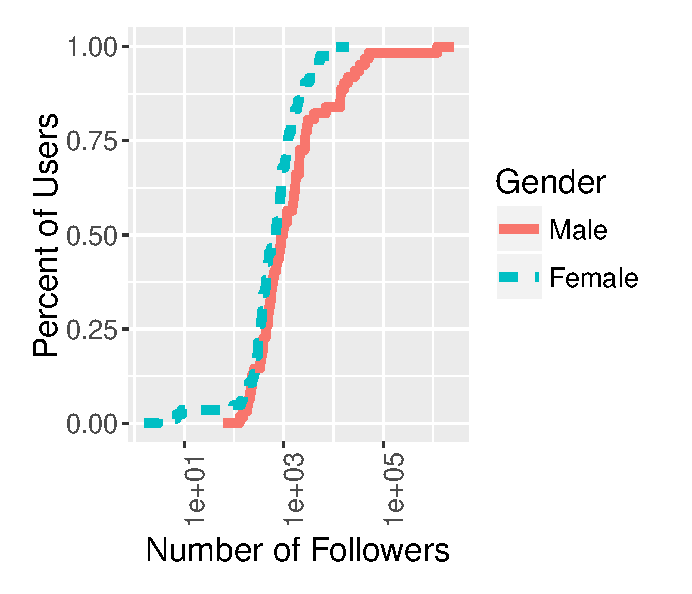
\includegraphics[width=\linewidth]{fig/census/followers_cdf_gender.eps}
    \caption{}
    \label{fig:followers_cdf_gender}
  \end{subfigure}
  \begin{subfigure}[b]{.21\textwidth}
    \centering
    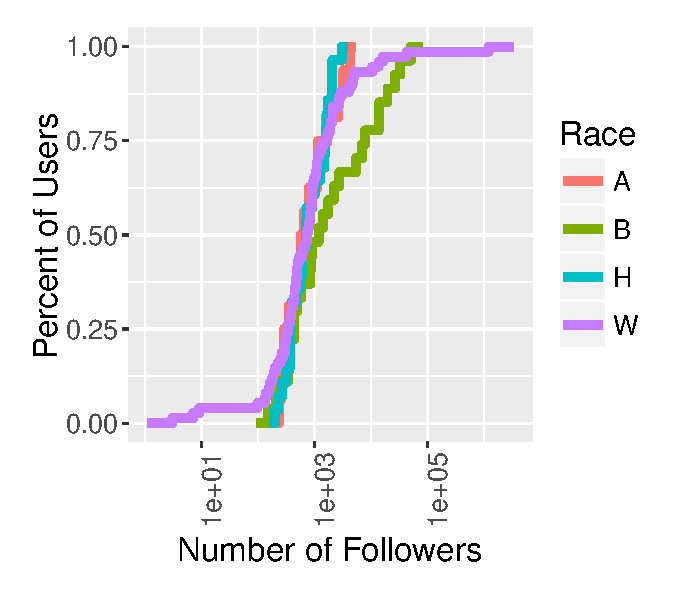
\includegraphics[width=\linewidth]{fig/census/followers_cdf_race.eps}
    \caption{}
    \label{fig:followers_cdf_race}
  \end{subfigure}

  \begin{subfigure}[b]{.21\textwidth}
    \centering
    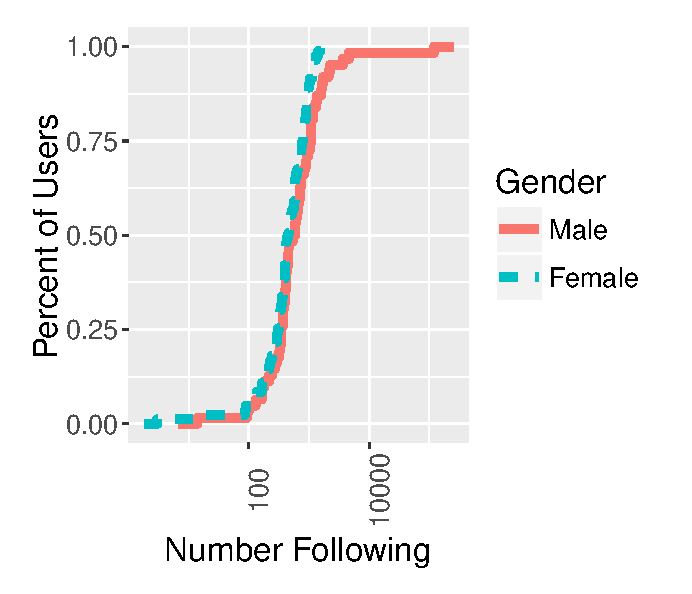
\includegraphics[width=\linewidth]{fig/census/following_cdf_gender.eps}
    \caption{}
    \label{fig:following_cdf_gender}
  \end{subfigure}
  \begin{subfigure}[b]{.21\textwidth}
    \centering
    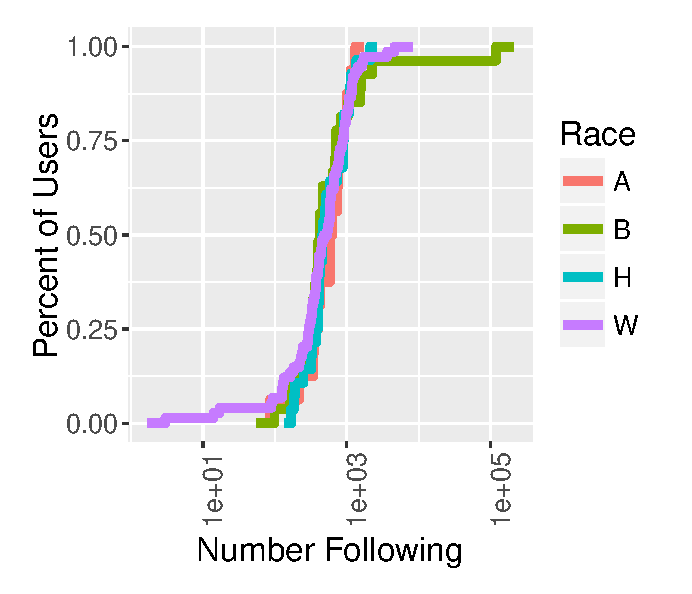
\includegraphics[width=\linewidth]{fig/census/following_cdf_race.eps}
    \caption{}
    \label{fig:following_cdf_race}
  \end{subfigure}
  \caption{}
  \label{fig:follow_cdf}
\end{figure}

We next compared several Instagram behaviors by demographic.
Figure~\ref{fig:face_cdf_gender} shows that women in our dataset typically have more faces in their photographs than men.
There appears to be more parity in number of faces for each of the considered racial groups, with Hispanics and Asians displaying slightly more faces in their photos.

We examine potential differences in the total number of photos posted by a user to their account in Figure~\ref{fig:numphoto_cdf}.
There does not appear to be a great difference for any particular group.

We investigate the relationship between gender, race, and following behavior in Figure~\ref{fig:follow_cdf} .
Instagram has a directional follower relationship, akin to that of Twitter.
If a user, Alice, follows Bob, it means that Alice will see updates from Bob in her feed.
Bob, however, will not see updates from Alice unless he decides to follow her.
Figures~\ref{fig:followers_cdf_gender} and~\ref{fig:following_cdf_gender} show differences in following behavior within our dataset for gender. 
It appears that men have more followers, and follow slightly more people.

In Figures~\ref{fig:followers_cdf_race} and~\ref{fig:following_cdf_race}, we see can make a few observations for following behavior among race in our dataset.
First, we see that the upper 50\% of Black users in our dataset have more followers than other groups, except for at the very top percentiles, where White users dominate.
At the highest percentiles, Black users \emph{follow} the most people.
% TODO: mention Black Twitter...
% http://www.slate.com/articles/technology/technology/2010/08/how_black_people_use_twitter.html
% Maybe http://dl.acm.org/citation.cfm?id=1963503
% duggan and smith: demo of key social networking platforms



\textbf{Methodology}
% Recognizing and labeling the faces present in each photo does not definitively tell us the gender or race of the user profile. 
The face recognition software only works at the level of a single photograph.
% This does not tell us the race or gender of the user on which these photographs appear.
We thus need to use an algorithm to go from the data of each picture to labeling an entire profile.
We rely on one main assumption: the owner of profile will appear in more photos than any other individual.

This assumption led us to test several different algorithms: 
\begin{itemize}
\item \textbf{Majority rule}: Count each face as a vote. 
  Profile is labeled with the gender (or race) with the most votes.
\item \textbf{Weighted majority rule}: Count each face as a vote.
  However, a face now gets as many votes as the confidence score.
  Thus, faces with lower confidence get lower weight.
  Profile is labeled with the gender (or race) with the most votes.
\item \textbf{Profile picture}: We simply take the result of the profile picture labeling.
\end{itemize}

Additionally, we applied a ``face weight" correction to all of these.
In a photo with three faces, only one of these faces could be the user.
It therefore might make sense to weight each face in this photo lower than in a photo with one face.
The face weight (fw) correction does just this, multiplying the weight of photo by the inverse of the number of faces in that photograph.
In our original example, the weight of each of the three faces would be multiplied by one third.
This is equivalent to averaging the gender or race (potentially with confidence scores) of all users in a photograph.


\textbf{Results}

\textbf{Gender}
Our human labelers categorized 76 profiles as Male and 94 as Female.
Running our three algorithms with and without the face weight correction, we obtained the following results:
\begin{itemize}
\item \textbf{Majority rule}: 85.1\%
\item \textbf{Weighted majority rule}: 85.7\%
\item \textbf{Majority Rule, FW}: 86.9\%
\item \textbf{Weighted Majority Rule, FW}: 87.5\%
\item \textbf{Profile picture}: 86.3\%
\end{itemize}

We observe that using the face weight correction improves the results for both algorithms.
Although profile pictures provide accurate information, only 70 out of 170 of these users had a profile picture that included a face.
For the remainder of this section, we will focus on the highest accuracy algorithm, weighted majority rule with FW.
A feature of this algorithm is that it outputs a probability for each user, enabling us to analyze the performance in more detail.
% \begin{figure}[!tbp]
%   \centering
%   \begin{minipage}[b]{0.4\textwidth}
%     \includegraphics[width=\textwidth]{flower1.jpg}
%     \caption{Flower one.}
%   \end{minipage}
%   \hfill
%   \begin{minipage}[b]{0.4\textwidth}
%     \includegraphics[width=\textwidth]{flower2.jpg}
%     \caption{Flower two.}
%   \end{minipage}
% \end{figure}

\begin{figure}[h]
  \centering
  \begin{minipage}{.21\textwidth}
    \centering
    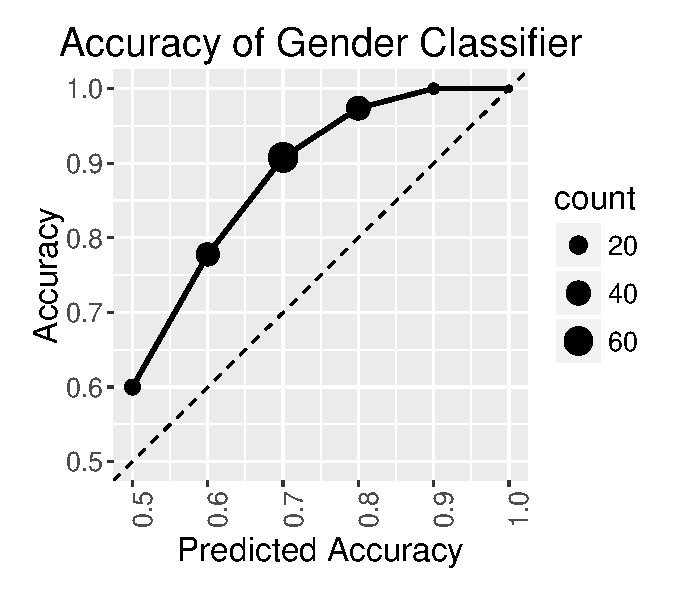
\includegraphics[width=\linewidth]{fig/census/accuracy_gender.eps}
    \caption{Predicted accuracy versus actual accuracy }
    \label{fig:accuracy_gender}
  \end{minipage}
  \begin{minipage}{.21\textwidth}
    \centering
    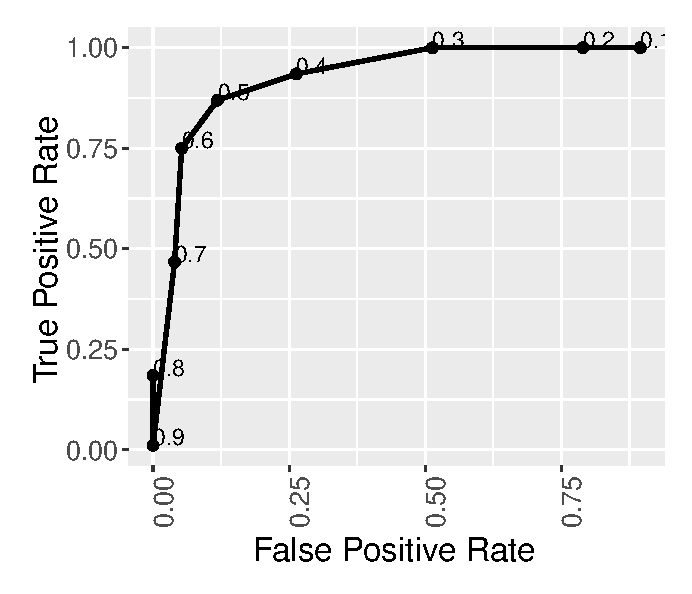
\includegraphics[width=\linewidth]{fig/census/roc_gender.eps}
    \caption{True positive versus false positive rate when labeling at various threshold levels.}
    \label{fig:roc_gender}
  \end{minipage}
  \caption{}
  \label{fig:accuracy_gender_all}
\end{figure}

\begin{figure}[h]
  \centering
  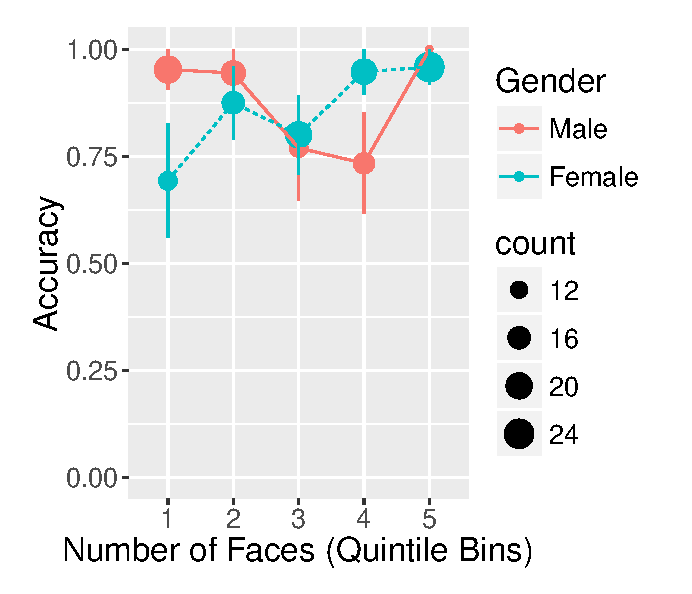
\includegraphics[width=.5\linewidth]{fig/census/facebin_gender.eps}
  \caption{Number of faces detected in first 100 photos vs. accuracy, by gender}
  \label{fig:facebin_gender}
\end{figure}
% TODO: add the boxplot thing in here, just because this looks bad right now

In Fig.~\ref{fig:accuracy_gender}, we group individuals on how what our algorithm predicts is the likelihood that that individual is female, and plot the accuracy within each group.
This shows us how well calibrated our algorithm is; if the output probability estimates are perfectly accurate, then half of the users with estimate 50\% should be female, and this plot should align on the 1:1 line.
Instead, we see that the line is above the diagonal, meaning our accuracy estimate is actually an underestimate.
Most likely, we could incorporate a prior probability into our algorithm to make it better calibrated.

In Fig.~\ref{fig:roc_gender}, we plot an ROC curve, showing the trade-off between accurate and inaccurate labelings when using a threshold on the algorithm's output probability.
For example, if we label as female all users with a probability of female over 60\%, around 75\% of female users would be correctly labeled, and we would exclude properly all but around 7\% of males.

In Fig.~\ref{fig:facebin_gender}, we observe that for users labeled female, as more faces are detected in their profiles, accuracy increases.
Perhaps counterintuitively, we see a dip for men, where male users with the 40-80\% most faces have much lower accuracy those in the bottom two quintiles, the bottom 40\%.
One possible hypothesis to explain this is that as some users add more faces, they will start to add a larger diversity of faces.
When this diversity increases, accuracy may decrease.
We leave the question of whether this is the mechanism open for later work.


\textbf{Race} \\

For race, 75 users were labeled White, 28 as Hispanic, 27 as Black, 16 as Asian, and 1 as other.
However, Face++ only labels users as Asian, Black, or White and will therefore always be incorrect on any of our users categorized as Hispanic or ``Other".
Thus, we'll present results both for all users, and for the reduced set of users labeled manually by our research assistants as Asian, Black, or White (``filtered").
Running our algorithms with and without the face weight correction, we obtained the following results:
\begin{itemize}
\item \textbf{Majority rule}: 64.4\% (all) 79.3\% (filtered)
\item \textbf{Weighted majority rule}: 66.2\% (all) 82.1\% (filtered)
\item \textbf{Majority Rule, FW}: 66.4\% 82.2\% (filtered)
\item \textbf{Weighted Majority Rule, FW}: 66.2\% (all), 82.1\% (filtered)
\item \textbf{Profile picture}: 57.1\% (all), 71.1\% (filtered)
\end{itemize}

On the users for which we have some hope of accuracy, the best algorithm achieves 82.2\% accuracy.
For the remainder of this section, we will constrain our results to the Weighted Majority algorithm, FW, due to the probabilities that it outputs and its nearly identital performance to the next best algorithm.
Additionally, we will look at some labelings as a binary classification problem between White users and Minority users.

% TODO: fix titles here
\begin{figure}[h]
  \centering
  \begin{minipage}{.21\textwidth}
    \centering
    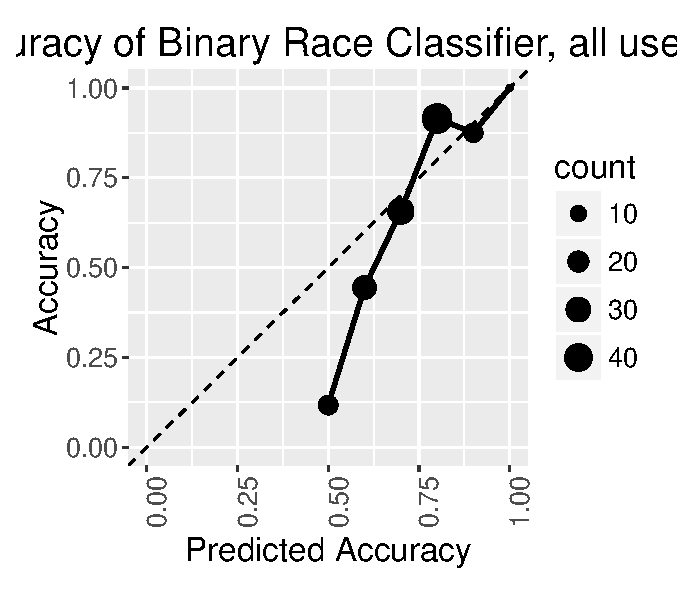
\includegraphics[width=\linewidth]{fig/census/accuracy_race_all.eps}
    % \caption{Predicted accuracy versus actual accuracy }
    \label{fig:accuracy_race_all}
  \end{minipage}
  \begin{minipage}{.21\textwidth}
    \centering
    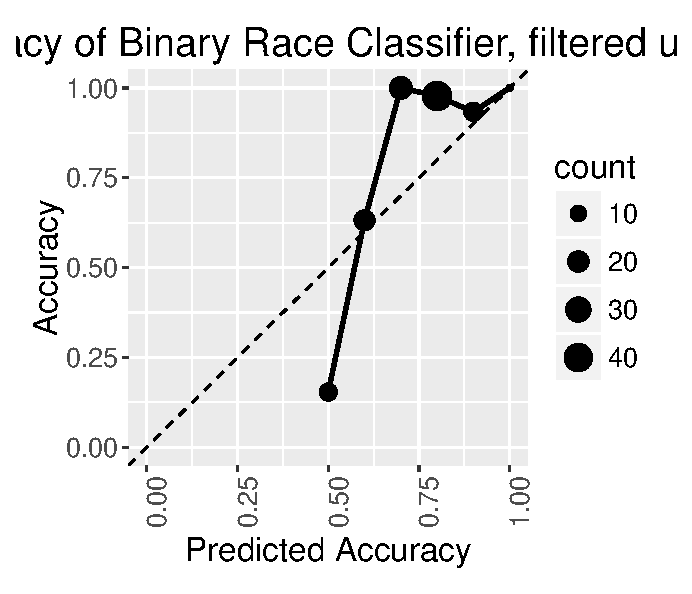
\includegraphics[width=\linewidth]{fig/census/accuracy_race_filtered.eps}
    % \caption{True positive versus false positive rate when labeling at various threshold levels.}
    \label{fig:accuracy_race_filtered}
  \end{minipage}
  % \caption{}
  \label{fig:accuracy_race}
\end{figure}

\begin{figure}[h]
  \centering
  \begin{minipage}{.21\textwidth}
    \centering
    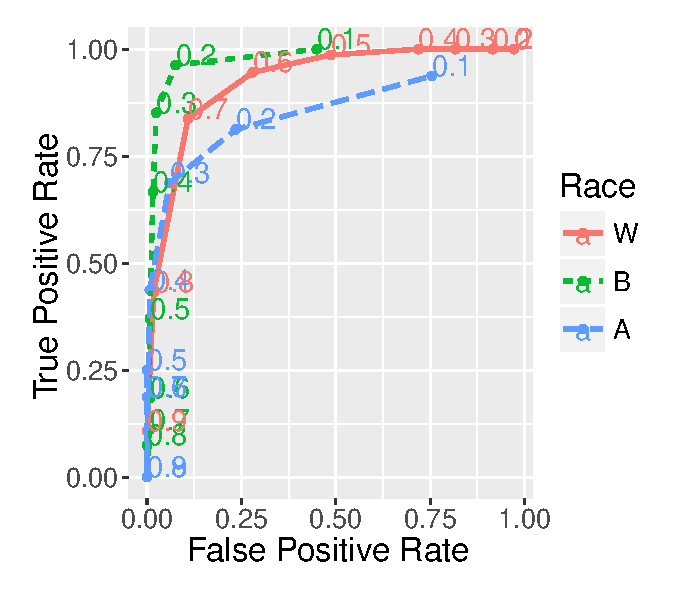
\includegraphics[width=\linewidth]{fig/census/roc_race.eps}
    % \caption{Predicted accuracy versus actual accuracy }
    \label{fig:roc_race}
  \end{minipage}
  \begin{minipage}{.21\textwidth}
    \centering
    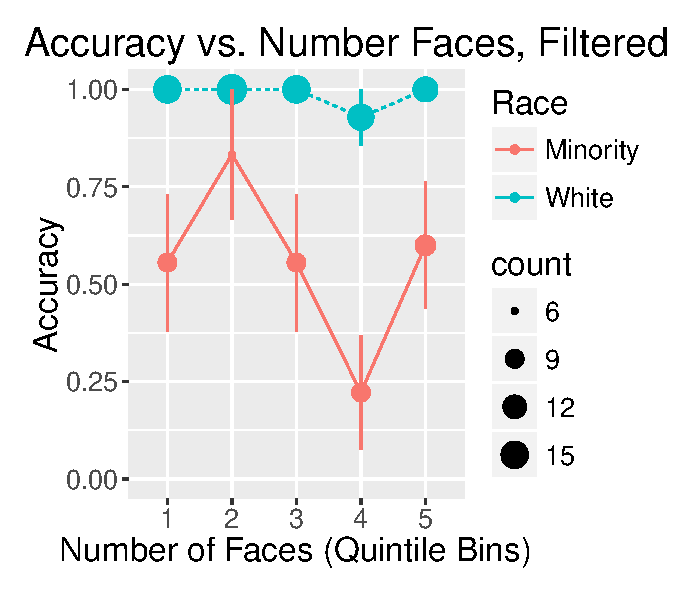
\includegraphics[width=\linewidth]{fig/census/facebin_race_filtered.eps}
    % \caption{True positive versus false positive rate when labeling at various threshold levels.}
    \label{fig:facebin_race_filtered}
  \end{minipage}
  \caption{}
  \label{fig:more_race}
\end{figure}

Based on Fig.~\ref{fig:accuracy_race}, the algorithm does not appear to be well-calibrated, both in being overconfident in the users with low probability estimations, and being underconfident in users with higher estimates.

An important aspect of demographic labeling is considering issues of the digital divide or disparate impact.
In Fig.~\ref{fig:more_race}, we see that accuracy is much lower on minorities than it is on White users.
Again, we see a lowering of accuracy as the number of faces increases, akin to the dip in accuracy Male users show in Fig.~\ref{fig:facebin_gender}.

\textbf{Discussion} \\
Among our dataset, we see some examples of differences in behavior.
For example, women tended to have more faces in their photos, and black users tended to have more followers.
A larger sample and careful statistical analysis should be taken to verify these results.
Applying machine learning to many more profiles could reveal, and possibly help explain, these and other differences in behaviors on Instagram.

In applying these techniques there are dangers of algorithmic bias.
The large difference in accuracy between white users and minority users is an example of this.
Our technique as it stands could suffer from this issue.
For example, users with more diverse faces in their profile (both gender and racially) may be harder to label.
Using a thresholding technique to only obtian high-accuracy users might leave only users who display strong homophily.

Further exascerbating the problem is that racial minority users actually \emph{decrease} in accuracy as there is more data about them, up to a certain point. 
Clearly more work is need to be done to understand this issue.
It may be important to consider the trade-offs here.
A more accurate algorithm may not be preferable to an algorithm that is equally accurate across demographic groups, and that behaves similarly in regards to the scaling of data.

% \section{Conclusion}
\textbf{Conclusion} \\
In this work, we've shown that computational vision techniques have some promise in becoming a valuable tool for demographers.
By combining facial recognition with the OSN Instagram, we've proven that the race and gender of users can be inferred with high precision and recall.

We see several important next steps to this work.
First, a larger scale verification of the results of this work should be obtained, with more users, aiming for diversity in many senses-- culturally, economically, racially, geographically, etc.
Such a verification should investigate the accuracy of the technique on various demographics in order to minimize algorithmic bias. 

Another direction is to use more powerful machine learning techniques on this problem.
For example, instead of naively incorporating all faces in a profile, a researcher could cluster faces based on a similarity score.
The largest cluster would most likely contain the users face.
Other facial recognition software packages, with a wider range of races, or with other features, could improve upon these results.

Finally, this technique could be used to engage in studies of various demographic groups and answer different questions.
Do different demographics use social networks in different ways?
What can we learn about interactiokn on the OSN between groups?
Combining demographic data with location data, we could additionally learn about immigration or human mobility.
